\documentclass[]{article}
\usepackage{lmodern}
\usepackage{amssymb,amsmath}
\usepackage{ifxetex,ifluatex}
\usepackage{fixltx2e} % provides \textsubscript
\ifnum 0\ifxetex 1\fi\ifluatex 1\fi=0 % if pdftex
  \usepackage[T1]{fontenc}
  \usepackage[utf8]{inputenc}
\else % if luatex or xelatex
  \ifxetex
    \usepackage{mathspec}
  \else
    \usepackage{fontspec}
  \fi
  \defaultfontfeatures{Ligatures=TeX,Scale=MatchLowercase}
\fi
% use upquote if available, for straight quotes in verbatim environments
\IfFileExists{upquote.sty}{\usepackage{upquote}}{}
% use microtype if available
\IfFileExists{microtype.sty}{%
\usepackage[]{microtype}
\UseMicrotypeSet[protrusion]{basicmath} % disable protrusion for tt fonts
}{}
\PassOptionsToPackage{hyphens}{url} % url is loaded by hyperref
\usepackage[unicode=true]{hyperref}
\hypersetup{
            pdftitle={range\_expansion},
            pdfauthor={Amanda Stahlke},
            pdfborder={0 0 0},
            breaklinks=true}
\urlstyle{same}  % don't use monospace font for urls
\usepackage[margin=1in]{geometry}
\usepackage{color}
\usepackage{fancyvrb}
\newcommand{\VerbBar}{|}
\newcommand{\VERB}{\Verb[commandchars=\\\{\}]}
\DefineVerbatimEnvironment{Highlighting}{Verbatim}{commandchars=\\\{\}}
% Add ',fontsize=\small' for more characters per line
\usepackage{framed}
\definecolor{shadecolor}{RGB}{248,248,248}
\newenvironment{Shaded}{\begin{snugshade}}{\end{snugshade}}
\newcommand{\KeywordTok}[1]{\textcolor[rgb]{0.13,0.29,0.53}{\textbf{#1}}}
\newcommand{\DataTypeTok}[1]{\textcolor[rgb]{0.13,0.29,0.53}{#1}}
\newcommand{\DecValTok}[1]{\textcolor[rgb]{0.00,0.00,0.81}{#1}}
\newcommand{\BaseNTok}[1]{\textcolor[rgb]{0.00,0.00,0.81}{#1}}
\newcommand{\FloatTok}[1]{\textcolor[rgb]{0.00,0.00,0.81}{#1}}
\newcommand{\ConstantTok}[1]{\textcolor[rgb]{0.00,0.00,0.00}{#1}}
\newcommand{\CharTok}[1]{\textcolor[rgb]{0.31,0.60,0.02}{#1}}
\newcommand{\SpecialCharTok}[1]{\textcolor[rgb]{0.00,0.00,0.00}{#1}}
\newcommand{\StringTok}[1]{\textcolor[rgb]{0.31,0.60,0.02}{#1}}
\newcommand{\VerbatimStringTok}[1]{\textcolor[rgb]{0.31,0.60,0.02}{#1}}
\newcommand{\SpecialStringTok}[1]{\textcolor[rgb]{0.31,0.60,0.02}{#1}}
\newcommand{\ImportTok}[1]{#1}
\newcommand{\CommentTok}[1]{\textcolor[rgb]{0.56,0.35,0.01}{\textit{#1}}}
\newcommand{\DocumentationTok}[1]{\textcolor[rgb]{0.56,0.35,0.01}{\textbf{\textit{#1}}}}
\newcommand{\AnnotationTok}[1]{\textcolor[rgb]{0.56,0.35,0.01}{\textbf{\textit{#1}}}}
\newcommand{\CommentVarTok}[1]{\textcolor[rgb]{0.56,0.35,0.01}{\textbf{\textit{#1}}}}
\newcommand{\OtherTok}[1]{\textcolor[rgb]{0.56,0.35,0.01}{#1}}
\newcommand{\FunctionTok}[1]{\textcolor[rgb]{0.00,0.00,0.00}{#1}}
\newcommand{\VariableTok}[1]{\textcolor[rgb]{0.00,0.00,0.00}{#1}}
\newcommand{\ControlFlowTok}[1]{\textcolor[rgb]{0.13,0.29,0.53}{\textbf{#1}}}
\newcommand{\OperatorTok}[1]{\textcolor[rgb]{0.81,0.36,0.00}{\textbf{#1}}}
\newcommand{\BuiltInTok}[1]{#1}
\newcommand{\ExtensionTok}[1]{#1}
\newcommand{\PreprocessorTok}[1]{\textcolor[rgb]{0.56,0.35,0.01}{\textit{#1}}}
\newcommand{\AttributeTok}[1]{\textcolor[rgb]{0.77,0.63,0.00}{#1}}
\newcommand{\RegionMarkerTok}[1]{#1}
\newcommand{\InformationTok}[1]{\textcolor[rgb]{0.56,0.35,0.01}{\textbf{\textit{#1}}}}
\newcommand{\WarningTok}[1]{\textcolor[rgb]{0.56,0.35,0.01}{\textbf{\textit{#1}}}}
\newcommand{\AlertTok}[1]{\textcolor[rgb]{0.94,0.16,0.16}{#1}}
\newcommand{\ErrorTok}[1]{\textcolor[rgb]{0.64,0.00,0.00}{\textbf{#1}}}
\newcommand{\NormalTok}[1]{#1}
\usepackage{graphicx,grffile}
\makeatletter
\def\maxwidth{\ifdim\Gin@nat@width>\linewidth\linewidth\else\Gin@nat@width\fi}
\def\maxheight{\ifdim\Gin@nat@height>\textheight\textheight\else\Gin@nat@height\fi}
\makeatother
% Scale images if necessary, so that they will not overflow the page
% margins by default, and it is still possible to overwrite the defaults
% using explicit options in \includegraphics[width, height, ...]{}
\setkeys{Gin}{width=\maxwidth,height=\maxheight,keepaspectratio}
\IfFileExists{parskip.sty}{%
\usepackage{parskip}
}{% else
\setlength{\parindent}{0pt}
\setlength{\parskip}{6pt plus 2pt minus 1pt}
}
\setlength{\emergencystretch}{3em}  % prevent overfull lines
\providecommand{\tightlist}{%
  \setlength{\itemsep}{0pt}\setlength{\parskip}{0pt}}
\setcounter{secnumdepth}{0}
% Redefines (sub)paragraphs to behave more like sections
\ifx\paragraph\undefined\else
\let\oldparagraph\paragraph
\renewcommand{\paragraph}[1]{\oldparagraph{#1}\mbox{}}
\fi
\ifx\subparagraph\undefined\else
\let\oldsubparagraph\subparagraph
\renewcommand{\subparagraph}[1]{\oldsubparagraph{#1}\mbox{}}
\fi

% set default figure placement to htbp
\makeatletter
\def\fps@figure{htbp}
\makeatother


\title{range\_expansion}
\author{Amanda Stahlke}
\date{3/6/2020}

\begin{document}
\maketitle

\begin{Shaded}
\begin{Highlighting}[]
\CommentTok{## convert this contig vcf to plink}
\ExtensionTok{module}\NormalTok{ load plink/1.90}

\ExtensionTok{plink}\NormalTok{ --bfile contig.populations.snps --set-missing-var-ids }\StringTok{"@_#"}\NormalTok{ --make-bed --out contig.populations.snps --allow-extra-chr}
\end{Highlighting}
\end{Shaded}

\begin{Shaded}
\begin{Highlighting}[]
\NormalTok{## range expansion}
\KeywordTok{library}\NormalTok{(rangeExpansion) ## Version: 0.0.0.9000}
\KeywordTok{library}\NormalTok{(dplyr)}
\end{Highlighting}
\end{Shaded}

\begin{verbatim}
## 
## Attaching package: 'dplyr'
\end{verbatim}

\begin{verbatim}
## The following objects are masked from 'package:stats':
## 
##     filter, lag
\end{verbatim}

\begin{verbatim}
## The following objects are masked from 'package:base':
## 
##     intersect, setdiff, setequal, union
\end{verbatim}

\begin{Shaded}
\begin{Highlighting}[]
\KeywordTok{library}\NormalTok{(snpStats) }\CommentTok{#1.32.0}
\end{Highlighting}
\end{Shaded}

\begin{verbatim}
## Loading required package: survival
\end{verbatim}

\begin{verbatim}
## Loading required package: Matrix
\end{verbatim}

\begin{Shaded}
\begin{Highlighting}[]
\KeywordTok{library}\NormalTok{(geosphere)}
\KeywordTok{library}\NormalTok{(rworldmap)}
\end{Highlighting}
\end{Shaded}

\begin{verbatim}
## Loading required package: sp
\end{verbatim}

\begin{verbatim}
## ### Welcome to rworldmap ###
\end{verbatim}

\begin{verbatim}
## For a short introduction type :   vignette('rworldmap')
\end{verbatim}

\begin{Shaded}
\begin{Highlighting}[]
\KeywordTok{library}\NormalTok{(ggplot2)}
\end{Highlighting}
\end{Shaded}

\subsection{make coords file}\label{make-coords-file}

\begin{Shaded}
\begin{Highlighting}[]
\NormalTok{snp.file <-}\StringTok{ "contig.populations.snps.bed"}
\NormalTok{geneticdat <-}\StringTok{ }\KeywordTok{load.plink.file}\NormalTok{(snp.file)}
\KeywordTok{nrow}\NormalTok{(geneticdat}\OperatorTok{$}\NormalTok{genotypes) }\CommentTok{# 154 individuals}
\end{Highlighting}
\end{Shaded}

\begin{verbatim}
## [1] 154
\end{verbatim}

\begin{Shaded}
\begin{Highlighting}[]
\NormalTok{id <-}\StringTok{ }\KeywordTok{data.frame}\NormalTok{(}\DataTypeTok{id =} \KeywordTok{rownames}\NormalTok{(geneticdat}\OperatorTok{$}\NormalTok{genotypes))}

\NormalTok{### make coords_file: id, longitude, latitude, outgroup, region, pop}
\NormalTok{sample_meta.dat <-}\StringTok{ }\KeywordTok{read.csv}\NormalTok{(}\StringTok{"../info/pop_metadata.csv"}\NormalTok{, }\DataTypeTok{header =} \OtherTok{TRUE}\NormalTok{, }\DataTypeTok{stringsAsFactors =} \OtherTok{FALSE}\NormalTok{)}
\NormalTok{ind_map <-}\StringTok{ }\KeywordTok{read.csv}\NormalTok{(}\StringTok{"intro_carinu_popmap.tsv"}\NormalTok{, }\DataTypeTok{sep =} \StringTok{"}\CharTok{\textbackslash{}t}\StringTok{"}\NormalTok{, }\DataTypeTok{header =}\NormalTok{ F, }\DataTypeTok{col.names =} \KeywordTok{c}\NormalTok{(}\StringTok{"id"}\NormalTok{, }\StringTok{"popID"}\NormalTok{))}
\KeywordTok{nrow}\NormalTok{(ind_map)}
\end{Highlighting}
\end{Shaded}

\begin{verbatim}
## [1] 154
\end{verbatim}

\begin{Shaded}
\begin{Highlighting}[]
\NormalTok{meta_ind <-}\StringTok{ }\KeywordTok{merge}\NormalTok{(sample_meta.dat, ind_map) }\OperatorTok
\StringTok{  }\KeywordTok{select}\NormalTok{(}\KeywordTok{c}\NormalTok{(id, Longitude, Latitude, popID))}

\NormalTok{meta_ind}\OperatorTok{$}\NormalTok{id <-}\StringTok{ }\KeywordTok{gsub}\NormalTok{(}\StringTok{'_rep'}\NormalTok{, }\StringTok{""}\NormalTok{, meta_ind}\OperatorTok{$}\NormalTok{id)}
\NormalTok{meta_ind}\OperatorTok{$}\NormalTok{id <-}\StringTok{ }\KeywordTok{gsub}\NormalTok{(}\StringTok{'_2019'}\NormalTok{, }\StringTok{""}\NormalTok{, meta_ind}\OperatorTok{$}\NormalTok{id)}

\NormalTok{## from population substructure}
\NormalTok{carinu_regions <-}\StringTok{ }\KeywordTok{data.frame}\NormalTok{(}\DataTypeTok{popID=}\KeywordTok{unique}\NormalTok{(meta_ind}\OperatorTok{$}\NormalTok{popID), }\DataTypeTok{region =} \KeywordTok{c}\NormalTok{(}\DecValTok{1}\NormalTok{, }\CommentTok{#11CO}
                                                                      \DecValTok{2}\NormalTok{, }\CommentTok{#12AZ}
                                                                      \DecValTok{1}\NormalTok{, }\CommentTok{#18TX}
                                                                      \DecValTok{1}\NormalTok{, }\CommentTok{#1WY}
                                                                      \DecValTok{1}\NormalTok{, }\CommentTok{#28NM}
                                                                      \DecValTok{1}\NormalTok{, }\CommentTok{#2CO}
                                                                      \DecValTok{2}\NormalTok{, }\CommentTok{#31NV}
                                                                      \DecValTok{2}\NormalTok{, }\CommentTok{#32UT}
                                                                      \DecValTok{2}\NormalTok{, }\CommentTok{#33NV}
                                                                      \DecValTok{2}\NormalTok{, }\CommentTok{#34UT}
                                                                      \DecValTok{1}\NormalTok{, }\CommentTok{#4CO}
                                                                      \DecValTok{1}\NormalTok{, }\CommentTok{#5CO }
                                                                      \DecValTok{1}\NormalTok{))}

\NormalTok{carinu_meta_regions <-}\StringTok{ }\KeywordTok{merge}\NormalTok{(meta_ind, carinu_regions)}


\KeywordTok{colnames}\NormalTok{(carinu_meta_regions)}
\end{Highlighting}
\end{Shaded}

\begin{verbatim}
## [1] "popID"     "id"        "Longitude" "Latitude"  "region"
\end{verbatim}

\begin{Shaded}
\begin{Highlighting}[]
\NormalTok{## col order  = id, longitude, latitude, pop, region}
\KeywordTok{colnames}\NormalTok{(carinu_meta_regions)[}\KeywordTok{c}\NormalTok{(}\DecValTok{1}\NormalTok{,}\DecValTok{3}\NormalTok{,}\DecValTok{4}\NormalTok{)] <-}\StringTok{ }\KeywordTok{c}\NormalTok{(}\StringTok{'pop'}\NormalTok{,}\StringTok{'longitude'}\NormalTok{, }\StringTok{'latitude'}\NormalTok{)}

\NormalTok{carinu_meta_regions <-}\StringTok{ }\NormalTok{carinu_meta_regions[,}\KeywordTok{c}\NormalTok{(}\StringTok{'id'}\NormalTok{,}\StringTok{'longitude'}\NormalTok{, }\StringTok{'latitude'}\NormalTok{, }\StringTok{'pop'}\NormalTok{, }\StringTok{'region'}\NormalTok{)]}
\NormalTok{carinu_meta_regions}
\end{Highlighting}
\end{Shaded}

\begin{verbatim}
##      id longitude latitude  pop region
## 1   F22   -104.16    37.34 11CO      1
## 2   F21   -104.16    37.34 11CO      1
## 3   E69   -104.16    37.34 11CO      1
## 4   F19   -104.16    37.34 11CO      1
## 5   F20   -104.16    37.34 11CO      1
## 6   E84   -104.16    37.34 11CO      1
## 7    F9   -104.16    37.34 11CO      1
## 8   E70   -104.16    37.34 11CO      1
## 9   E82   -104.16    37.34 11CO      1
## 10  F10   -104.16    37.34 11CO      1
## 11  E94   -104.16    37.34 11CO      1
## 12  E92   -104.16    37.34 11CO      1
## 13  E60   -114.64    35.12 12AZ      2
## 14  E65   -114.64    35.12 12AZ      2
## 15  E67   -114.64    35.12 12AZ      2
## 16  E59   -114.64    35.12 12AZ      2
## 17  F17   -114.64    35.12 12AZ      2
## 18  F18   -114.64    35.12 12AZ      2
## 19  F23   -114.64    35.12 12AZ      2
## 20  F24   -114.64    35.12 12AZ      2
## 21   F4   -114.64    35.12 12AZ      2
## 22   F5   -114.64    35.12 12AZ      2
## 23  E78   -114.64    35.12 12AZ      2
## 24  F15   -114.64    35.12 12AZ      2
## 25  E68   -114.64    35.12 12AZ      2
## 26  E77   -114.64    35.12 12AZ      2
## 27  F16   -114.64    35.12 12AZ      2
## 28  H65   -103.48    31.49 18TX      1
## 29  H66   -103.48    31.49 18TX      1
## 30  E38   -108.18    44.86  1WY      1
## 31   E4   -108.18    44.86  1WY      1
## 32  E47   -108.18    44.86  1WY      1
## 33  E48   -108.18    44.86  1WY      1
## 34  E49   -108.18    44.86  1WY      1
## 35  E50   -108.18    44.86  1WY      1
## 36  E25   -108.18    44.86  1WY      1
## 37  E26   -108.18    44.86  1WY      1
## 38  E27   -108.18    44.86  1WY      1
## 39  E28   -108.18    44.86  1WY      1
## 40   E3   -108.18    44.86  1WY      1
## 41  E35   -108.18    44.86  1WY      1
## 42  E36   -108.18    44.86  1WY      1
## 43  E37   -108.18    44.86  1WY      1
## 44  E15   -108.18    44.86  1WY      1
## 45   E1   -108.18    44.86  1WY      1
## 46  E13   -108.18    44.86  1WY      1
## 47   H8   -103.69    35.19 28NM      1
## 48  G18   -103.69    35.19 28NM      1
## 49   G7   -103.69    35.19 28NM      1
## 50   G8   -103.69    35.19 28NM      1
## 51  F91   -103.69    35.19 28NM      1
## 52  G17   -103.69    35.19 28NM      1
## 53  H30   -104.61    38.34  2CO      1
## 54  H31   -104.61    38.34  2CO      1
## 55  H32   -104.61    38.34  2CO      1
## 56  H29   -104.61    38.34  2CO      1
## 57  H43   -104.61    38.34  2CO      1
## 58  G89   -104.61    38.34  2CO      1
## 59  G90   -104.61    38.34  2CO      1
## 60   H4   -104.61    38.34  2CO      1
## 61  H13   -104.61    38.34  2CO      1
## 62  H14   -104.61    38.34  2CO      1
## 63  H15   -104.61    38.34  2CO      1
## 64  H16   -104.61    38.34  2CO      1
## 65   H7   -104.61    38.34  2CO      1
## 66  H46   -104.61    38.34  2CO      1
## 67  H44   -104.61    38.34  2CO      1
## 68  H45   -104.61    38.34  2CO      1
## 69  G92   -104.61    38.34  2CO      1
## 70   H5   -104.61    38.34  2CO      1
## 71   H6   -104.61    38.34  2CO      1
## 72  F12   -114.26    36.69 31NV      2
## 73  F13   -114.26    36.69 31NV      2
## 74  F14   -114.26    36.69 31NV      2
## 75   F1   -114.26    36.69 31NV      2
## 76  F11   -114.26    36.69 31NV      2
## 77  E95   -114.26    36.69 31NV      2
## 78   F2   -114.26    36.69 31NV      2
## 79  E34   -113.58    37.07 32UT      2
## 80  E43   -113.58    37.07 32UT      2
## 81  E46   -113.58    37.07 32UT      2
## 82  E55   -113.58    37.07 32UT      2
## 83  E45   -113.58    37.07 32UT      2
## 84  E33   -113.58    37.07 32UT      2
## 85  E10   -113.58    37.07 32UT      2
## 86  E44   -113.58    37.07 32UT      2
## 87  E32   -113.58    37.07 32UT      2
## 88  E57   -113.58    37.07 32UT      2
## 89  E58   -113.58    37.07 32UT      2
## 90  E11   -113.58    37.07 32UT      2
## 91  E56   -113.58    37.07 32UT      2
## 92  E31   -113.58    37.07 32UT      2
## 93  E21   -113.58    37.07 32UT      2
## 94  E22   -113.58    37.07 32UT      2
## 95   E9   -113.58    37.07 32UT      2
## 96  E12   -113.58    37.07 32UT      2
## 97  E24   -113.58    37.07 32UT      2
## 98  E23   -113.58    37.07 32UT      2
## 99  E75   -114.40    36.38 33NV      2
## 100 E86   -114.40    36.38 33NV      2
## 101 E87   -114.40    36.38 33NV      2
## 102 E85   -114.40    36.38 33NV      2
## 103 E63   -114.40    36.38 33NV      2
## 104 E64   -114.40    36.38 33NV      2
## 105 E76   -114.40    36.38 33NV      2
## 106 E61   -114.40    36.38 33NV      2
## 107 E62   -114.40    36.38 33NV      2
## 108 E18   -112.93    39.23 34UT      2
## 109 E17   -112.93    39.23 34UT      2
## 110 E39   -112.93    39.23 34UT      2
## 111 E40   -112.93    39.23 34UT      2
## 112 E41   -112.93    39.23 34UT      2
## 113 E42   -112.93    39.23 34UT      2
## 114  E5   -112.93    39.23 34UT      2
## 115 E51   -112.93    39.23 34UT      2
## 116 E52   -112.93    39.23 34UT      2
## 117 E53   -112.93    39.23 34UT      2
## 118  E7   -112.93    39.23 34UT      2
## 119  E8   -112.93    39.23 34UT      2
## 120 E90   -112.93    39.23 34UT      2
## 121 E19   -112.93    39.23 34UT      2
## 122 E20   -112.93    39.23 34UT      2
## 123 E54   -112.93    39.23 34UT      2
## 124 H51   -103.25    38.26  4CO      1
## 125 H53   -103.25    38.26  4CO      1
## 126 H59   -103.25    38.26  4CO      1
## 127 H52   -103.25    38.26  4CO      1
## 128 H37   -103.25    38.26  4CO      1
## 129 H54   -103.25    38.26  4CO      1
## 130 H40   -103.25    38.26  4CO      1
## 131 H39   -103.25    38.26  4CO      1
## 132 H60   -103.25    38.26  4CO      1
## 133 H62   -103.25    38.26  4CO      1
## 134 H38   -103.25    38.26  4CO      1
## 135 F39   -103.42    37.70  5CO      1
## 136 F38   -103.42    37.70  5CO      1
## 137 F52   -103.42    37.70  5CO      1
## 138 F51   -103.42    37.70  5CO      1
## 139 F26   -103.42    37.70  5CO      1
## 140 F27   -103.42    37.70  5CO      1
## 141 F50   -103.42    37.70  5CO      1
## 142 F25   -103.42    37.70  5CO      1
## 143 F73   -103.42    37.70  5CO      1
## 144 F74   -103.42    37.70  5CO      1
## 145 F49   -103.42    37.70  5CO      1
## 146 F60   -103.42    37.70  5CO      1
## 147 F37   -103.42    37.70  5CO      1
## 148 F61   -103.42    37.70  5CO      1
## 149 F59   -103.42    37.70  5CO      1
## 150 F28   -103.42    37.70  5CO      1
## 151 F72   -103.42    37.70  5CO      1
## 152 F62   -103.42    37.70  5CO      1
## 153 F71   -103.42    37.70  5CO      1
## 154 G47   -101.08    37.99  6KS      1
\end{verbatim}

\begin{Shaded}
\begin{Highlighting}[]
\NormalTok{xlen =}\StringTok{ }\KeywordTok{max}\NormalTok{(carinu_meta_regions}\OperatorTok{$}\NormalTok{longitude)}\OperatorTok{-}\KeywordTok{min}\NormalTok{(carinu_meta_regions}\OperatorTok{$}\NormalTok{longitude) }\OperatorTok{+}\StringTok{ }\DecValTok{10}

\NormalTok{ylen =}\StringTok{ }\KeywordTok{max}\NormalTok{(carinu_meta_regions}\OperatorTok{$}\NormalTok{latitude)}\OperatorTok{-}\KeywordTok{min}\NormalTok{(carinu_meta_regions}\OperatorTok{$}\NormalTok{latitude) }\OperatorTok{+}\DecValTok{10}

\KeywordTok{write.csv}\NormalTok{(carinu_meta_regions, }\StringTok{"carinu_meta_regions.csv"}\NormalTok{, }
          \DataTypeTok{quote =}\NormalTok{ F, }\DataTypeTok{row.names =}\NormalTok{ F)}
\end{Highlighting}
\end{Shaded}

\begin{Shaded}
\begin{Highlighting}[]
\NormalTok{snp.file <-}\StringTok{ "contig.populations.snps.bed"} \CommentTok{# should be renamed }
\NormalTok{carinu_coords.file <-}\StringTok{ "carinu_meta_regions.csv"}
\NormalTok{regions_to_analyze <-}\StringTok{ }\KeywordTok{list}\NormalTok{(}\OtherTok{NULL}\NormalTok{,}
                           \StringTok{"1"}\NormalTok{, }
                           \StringTok{"2"}\NormalTok{,}
                           \KeywordTok{c}\NormalTok{(}\StringTok{"1"}\NormalTok{, }\StringTok{"2"}\NormalTok{))}
\NormalTok{ploidy <-}\StringTok{ }\DecValTok{2} \CommentTok{#diploid individuals}

\NormalTok{raw.data <-}\StringTok{ }\KeywordTok{load.data}\NormalTok{(}\DataTypeTok{plink.file =}\NormalTok{ snp.file, }\DataTypeTok{coords.file =}\NormalTok{ carinu_coords.file, }\DataTypeTok{sep =} \StringTok{","}\NormalTok{, }\DataTypeTok{ploidy=}\NormalTok{ploidy)}

\NormalTok{pop <-}\StringTok{ }\KeywordTok{make.pop}\NormalTok{(raw.data, ploidy)}

\NormalTok{psi <-}\StringTok{ }\KeywordTok{get.all.psi}\NormalTok{(pop)}

\NormalTok{results <-}\StringTok{ }\KeywordTok{run.regions}\NormalTok{(}\DataTypeTok{region=}\NormalTok{regions_to_analyze, }\DataTypeTok{psi =}\NormalTok{ psi,  }\DataTypeTok{pop=}\NormalTok{pop, }\DataTypeTok{xlen=}\DecValTok{25}\NormalTok{, }\DataTypeTok{ylen=}\DecValTok{25}\NormalTok{)}
\end{Highlighting}
\end{Shaded}

\begin{verbatim}
## [1] "fid"     "default"
## [1] "plots/orig..default.25.pdf"
## [1] "fid"     "default"
## [1] "plots/orig.1.default.25.pdf"
## [1] "fid"     "default"
## [1] "plots/orig.2.default.25.pdf"
## [1] "fid"     "default"
## [1] "plots/orig.1+2.default.25.pdf"
\end{verbatim}

\begin{Shaded}
\begin{Highlighting}[]
\NormalTok{results_summary <-}\StringTok{ }\KeywordTok{summary}\NormalTok{(results)}

\KeywordTok{rbind}\NormalTok{(}\DataTypeTok{orgin_1 =} \KeywordTok{as.data.frame}\NormalTok{(results_summary}\OperatorTok{$}\StringTok{`}\DataTypeTok{1}\StringTok{`}\NormalTok{), }
           \DataTypeTok{origin_2 =} \KeywordTok{as.data.frame}\NormalTok{(results_summary}\OperatorTok{$}\StringTok{`}\DataTypeTok{2}\StringTok{`}\NormalTok{),}
           \DataTypeTok{origin_1_2 =} \KeywordTok{as.data.frame}\NormalTok{(results_summary}\OperatorTok{$}\StringTok{`}\DataTypeTok{1+2}\StringTok{`}\NormalTok{))}
\end{Highlighting}
\end{Shaded}

\begin{verbatim}
##            longitude latitude            q        r1       r10      r100
## orgin_1      -108.18 44.86000 2.458967e-05 0.9999508 0.9995084 0.9951061
## origin_2     -114.64 35.97625 1.344329e-04 0.9997312 0.9973186 0.9738174
## origin_1_2   -101.08 42.63167 9.224930e-05 0.9998155 0.9981584 0.9818844
##                   d1        rsq         pval
## orgin_1    205.39133 0.08987113 6.659315e+02
## origin_2    37.56897 0.47128097 1.697544e+02
## origin_1_2  54.74844 0.42174052 7.613144e-07
\end{verbatim}

\begin{Shaded}
\begin{Highlighting}[]
\KeywordTok{plot.origin.result.list}\NormalTok{(results)}
\end{Highlighting}
\end{Shaded}

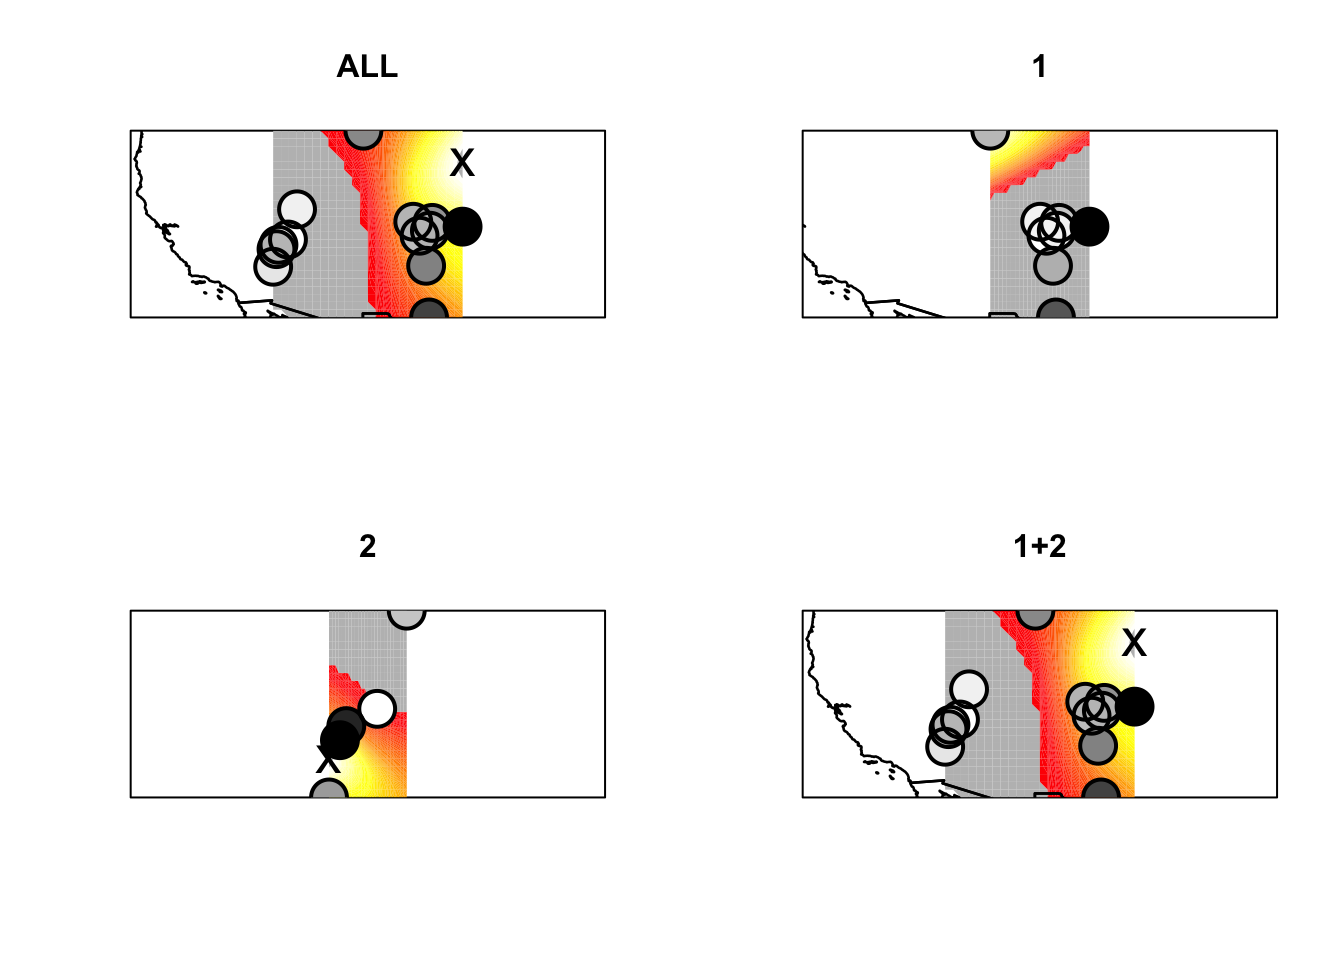
\includegraphics{range_expansion_files/figure-latex/all_intro_carinu_run-1.pdf}

\subsection{psi is directionality
index}\label{psi-is-directionality-index}

\begin{Shaded}
\begin{Highlighting}[]
\NormalTok{my_psi <-}\StringTok{ }\KeywordTok{as.matrix}\NormalTok{(psi)}
\KeywordTok{rownames}\NormalTok{(my_psi) <-}\StringTok{ }\NormalTok{pop}\OperatorTok{$}\NormalTok{coords}\OperatorTok{$}\NormalTok{pop}
\KeywordTok{colnames}\NormalTok{(my_psi) <-}\StringTok{ }\NormalTok{pop}\OperatorTok{$}\NormalTok{coords}\OperatorTok{$}\NormalTok{pop}

\NormalTok{melted_cormat <-}\StringTok{ }\NormalTok{reshape2}\OperatorTok{::}\KeywordTok{melt}\NormalTok{(my_psi, }\DataTypeTok{na.rm =} \OtherTok{TRUE}\NormalTok{)}
\NormalTok{melted_cormat <-}\StringTok{ }\NormalTok{melted_cormat[}\KeywordTok{order}\NormalTok{(melted_cormat}\OperatorTok{$}\NormalTok{value, }\DataTypeTok{decreasing =} \OtherTok{TRUE}\NormalTok{),]}
\NormalTok{melted_cormat}\OperatorTok{$}\NormalTok{Var1 <-}\StringTok{ }\KeywordTok{factor}\NormalTok{(melted_cormat}\OperatorTok{$}\NormalTok{Var1, }\DataTypeTok{levels=}\KeywordTok{unique}\NormalTok{(melted_cormat}\OperatorTok{$}\NormalTok{Var1[}\KeywordTok{order}\NormalTok{(melted_cormat}\OperatorTok{$}\NormalTok{value)]))}
\NormalTok{melted_cormat}\OperatorTok{$}\NormalTok{Var2 <-}\StringTok{ }\KeywordTok{factor}\NormalTok{(melted_cormat}\OperatorTok{$}\NormalTok{Var2, }\DataTypeTok{levels=}\KeywordTok{unique}\NormalTok{(melted_cormat}\OperatorTok{$}\NormalTok{Var2[}\KeywordTok{order}\NormalTok{(melted_cormat}\OperatorTok{$}\NormalTok{value)]))}

\CommentTok{# library(ggplot2)}
\KeywordTok{ggplot}\NormalTok{(}\DataTypeTok{data =}\NormalTok{ melted_cormat, }\KeywordTok{aes}\NormalTok{(Var1, Var2, }\DataTypeTok{fill =}\NormalTok{ value))}\OperatorTok{+}
\StringTok{  }\KeywordTok{geom_tile}\NormalTok{(}\DataTypeTok{color =} \StringTok{"white"}\NormalTok{)}\OperatorTok{+}
\StringTok{  }\KeywordTok{scale_fill_gradient2}\NormalTok{(}\DataTypeTok{low =} \StringTok{"blue"}\NormalTok{, }\DataTypeTok{high =} \StringTok{"red"}\NormalTok{, }\DataTypeTok{mid =} \StringTok{"white"}\NormalTok{, }
                       \DataTypeTok{midpoint =} \DecValTok{0}\NormalTok{, }\DataTypeTok{limit =} \KeywordTok{c}\NormalTok{(}\OperatorTok{-}\NormalTok{.}\DecValTok{3}\NormalTok{,.}\DecValTok{3}\NormalTok{), }\DataTypeTok{space =} \StringTok{"Lab"}\NormalTok{, }
                       \DataTypeTok{name=}\StringTok{"Psi"}\NormalTok{) }\OperatorTok{+}
\StringTok{  }\KeywordTok{xlab}\NormalTok{(}\StringTok{"Psi_1"}\NormalTok{) }\OperatorTok{+}
\StringTok{  }\KeywordTok{ylab}\NormalTok{(}\StringTok{"Psi_2"}\NormalTok{) }\OperatorTok{+}
\StringTok{  }\KeywordTok{theme_minimal}\NormalTok{()}\OperatorTok{+}\StringTok{ }
\StringTok{  }\KeywordTok{theme}\NormalTok{(}\DataTypeTok{axis.text.x =} \KeywordTok{element_text}\NormalTok{(}\DataTypeTok{angle =} \DecValTok{45}\NormalTok{, }\DataTypeTok{vjust =} \DecValTok{1}\NormalTok{, }
                                   \DataTypeTok{size =} \DecValTok{12}\NormalTok{, }\DataTypeTok{hjust =} \DecValTok{1}\NormalTok{))}\OperatorTok{+}
\StringTok{  }\KeywordTok{coord_fixed}\NormalTok{()}
\end{Highlighting}
\end{Shaded}

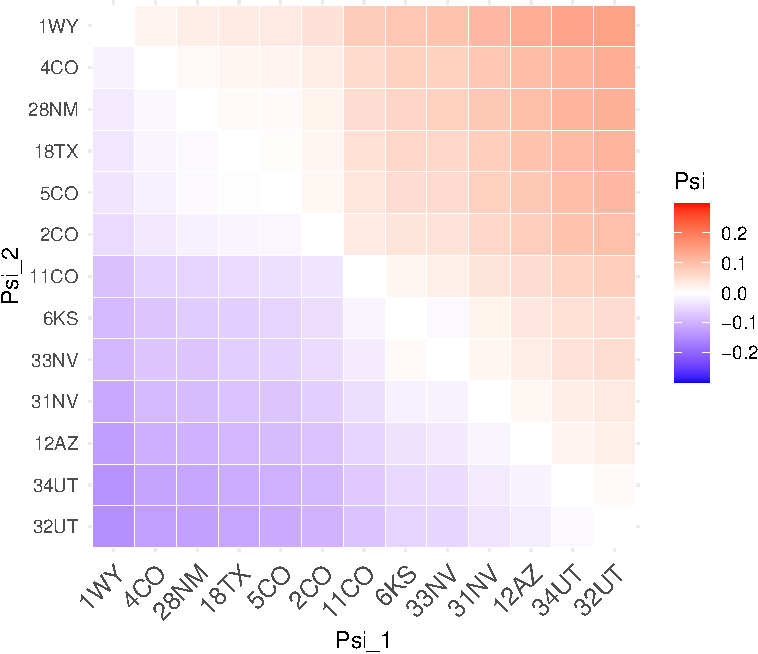
\includegraphics{range_expansion_files/figure-latex/psi-1.pdf}

\begin{Shaded}
\begin{Highlighting}[]
\KeywordTok{ggsave}\NormalTok{(}\StringTok{"range_expansion_psi.jpeg"}\NormalTok{, }\DataTypeTok{dpi =} \DecValTok{300}\NormalTok{)}
\end{Highlighting}
\end{Shaded}

\begin{verbatim}
## Saving 6.5 x 4.5 in image
\end{verbatim}

\subsection{Try again with samples only along virgin river
expansion}\label{try-again-with-samples-only-along-virgin-river-expansion}

\begin{Shaded}
\begin{Highlighting}[]
\NormalTok{snp.file <-}\StringTok{ "virgin-river.contig.populations.snps"}
\NormalTok{geneticdat <-}\StringTok{ }\KeywordTok{load.plink.file}\NormalTok{(snp.file)}
\KeywordTok{nrow}\NormalTok{(geneticdat}\OperatorTok{$}\NormalTok{genotypes) }\CommentTok{# 67 individuals}
\end{Highlighting}
\end{Shaded}

\begin{verbatim}
## [1] 67
\end{verbatim}

\begin{Shaded}
\begin{Highlighting}[]
\NormalTok{id <-}\StringTok{ }\KeywordTok{data.frame}\NormalTok{(}\DataTypeTok{id =} \KeywordTok{rownames}\NormalTok{(geneticdat}\OperatorTok{$}\NormalTok{genotypes))}

\NormalTok{ploidy <-}\StringTok{ }\DecValTok{2} \CommentTok{#diploid individuals}

\NormalTok{### make coords_file: id, longitude, latitude, outgroup, region, pop}
\NormalTok{sample_meta.dat}
\end{Highlighting}
\end{Shaded}

\begin{verbatim}
##         popID                                                            Name
## 1        46CH                                                    Bitun, China
## 2         1WY                                                          Lovell
## 3        44GR                                            Delta Aksiou, Greece
## 4        43GR                                                  Posidi, Greece
## 5        34UT                                                           Delta
## 6         2CO                                                  Fountain Creek
## 7         4CO                                   Adobe Reservoir (Blue Lake)\n
## 8         6KS                                                 W Finney County
## 9         5CO                                                       SE corner
## 10       11CO                                                       Wilkinson
## 11       32UT                                                      St. George
## 12        8OK                                                          Guymon
## 13       31NV                                       Virgin River - Gold Butte
## 14       33NV                                          Lake Mead, Stewarts Pt
## 15       39CR                                       Panaramnos, Crete, Greece
## 16       38CR                                                       Crete, GR
## 17       37CR                                         Rethimno, Crete, Greece
## 18       40CR                                           Sfkaki, Crete, Greece
## 19       41CR                                          Plakias, Crete, Greece
## 20       28NM                                                  Tucumcari Lake
## 21       12AZ                                                        Big Bend
## 22       42CR                                      Agia Galini, Crete, Greece
## 23       26NM                                                     Lake Sumner
## 24       27NM                                                       Roswell E
## 25       15TX                                                       NE Post\n
## 26       19TX                                                       Aspermont
## 27       21NM                                        Artesia Wildlife Reserve
## 28       16TX                                                  Lake JB Thomas
## 29       20NM                                                        Malaga\n
## 30       18TX                                                            Orla
## 31       52TX                                                        Tornillo
## 32       50TX                                                    Presidio Hwy
## 33       51TX                                             CO Canyon Boat Ramp
## 34       47TX Rio Grande Village - from T. cheninsis x T. ramosissima hybrids
## 35       49TX                                                     Santa Elana
## 36 CARINA_LAB                                       D. carinata Lab Culture\n
## 37    SUB_LAB                                     D. sublineata Lab Culture\n
##    Latitude Longitude Date.Collected Order                   Grp
## 1     47.30     87.75         7/3/16     1            carinulata
## 2     44.86   -108.18         9/3/14     2            carinulata
## 3     40.55     22.74         7/6/15    14       native_elongata
## 4     39.97     23.37         7/6/15    15       native_elongata
## 5     39.23   -112.93       10/15/14     3            carinulata
## 6     38.34   -104.61         9/2/14     4            carinulata
## 7     38.26   -103.25         9/4/14     5            carinulata
## 8     37.99   -101.08         8/8/14    22 potential_hybrid_zone
## 9     37.70   -103.42        8/21/14     6            carinulata
## 10    37.34   -104.16        9/18/14     7            carinulata
## 11    37.07   -113.58       10/15/14     8            carinulata
## 12    36.70   -101.55        9/16/14    23 potential_hybrid_zone
## 13    36.69   -114.26       10/15/14     9            carinulata
## 14    36.38   -114.40       10/15/14    10            carinulata
## 15    35.42     24.68         7/4/15    16       native_elongata
## 16    35.42     24.69         7/4/15    17       native_elongata
## 17    35.37     24.47         7/2/15    18       native_elongata
## 18    35.35     24.34         7/4/15    19       native_elongata
## 19    35.19     24.40         7/4/15    20       native_elongata
## 20    35.19   -103.69        10/6/14    24 potential_hybrid_zone
## 21    35.12   -114.64        9/18/14    11            carinulata
## 22    35.10     24.69         7/4/15    21       native_elongata
## 23    34.15   -104.48        9/29/14    25 potential_hybrid_zone
## 24    33.40   -104.41        9/29/14    26 potential_hybrid_zone
## 25    33.32   -101.26        9/26/14    27 potential_hybrid_zone
## 26    33.17   -100.24        9/27/14    28 potential_hybrid_zone
## 27    32.98   -104.44        10/7/14    29 potential_hybrid_zone
## 28    32.61   -101.22        9/26/14    30 potential_hybrid_zone
## 29    32.22   -104.08        9/27/14    31 potential_hybrid_zone
## 30    31.49   -103.48        9/27/14    32 potential_hybrid_zone
## 31    31.44   -106.09         8/3/17    33 potential_hybrid_zone
## 32    29.34   -104.07         8/3/17    34 potential_hybrid_zone
## 33    29.34   -104.06         8/3/17    35 potential_hybrid_zone
## 34    29.18   -102.96         8/3/17    36 potential_hybrid_zone
## 35    29.16   -103.60         8/3/17    37 potential_hybrid_zone
## 36       NA        NA                   12                   lab
## 37       NA        NA                   13                   lab
##                      cat
## 1                 native
## 2       original_release
## 3                 native
## 4                 native
## 5       original_release
## 6       original_release
## 7   carinulata_expansion
## 8  potential_hybrid_zone
## 9   carinulata_expansion
## 10  carinulata_expansion
## 11  carinulata_expansion
## 12 potential_hybrid_zone
## 13  carinulata_expansion
## 14  carinulata_expansion
## 15                native
## 16                native
## 17                native
## 18                native
## 19                native
## 20 potential_hybrid_zone
## 21  carinulata_expansion
## 22                native
## 23 potential_hybrid_zone
## 24 potential_hybrid_zone
## 25 potential_hybrid_zone
## 26 potential_hybrid_zone
## 27 potential_hybrid_zone
## 28      original_release
## 29 potential_hybrid_zone
## 30 potential_hybrid_zone
## 31 potential_hybrid_zone
## 32 potential_hybrid_zone
## 33 potential_hybrid_zone
## 34      original_release
## 35 potential_hybrid_zone
## 36                   lab
## 37                   lab
\end{verbatim}

\begin{Shaded}
\begin{Highlighting}[]
\NormalTok{ind_map <-}\StringTok{ }\KeywordTok{read.csv}\NormalTok{(}\StringTok{"intro_carinu_popmap.tsv"}\NormalTok{, }\DataTypeTok{sep =} \StringTok{"}\CharTok{\textbackslash{}t}\StringTok{"}\NormalTok{, }\DataTypeTok{header =}\NormalTok{ F, }\DataTypeTok{col.names =} \KeywordTok{c}\NormalTok{(}\StringTok{"id"}\NormalTok{, }\StringTok{"popID"}\NormalTok{))}
\NormalTok{ind_map}\OperatorTok{$}\NormalTok{id <-}\StringTok{ }\KeywordTok{gsub}\NormalTok{(}\StringTok{'_rep'}\NormalTok{, }\StringTok{""}\NormalTok{, ind_map}\OperatorTok{$}\NormalTok{id)}
\NormalTok{ind_map}\OperatorTok{$}\NormalTok{id <-}\StringTok{ }\KeywordTok{gsub}\NormalTok{(}\StringTok{'_2019'}\NormalTok{, }\StringTok{""}\NormalTok{, ind_map}\OperatorTok{$}\NormalTok{id)}

\NormalTok{ind_map <-}\StringTok{ }\KeywordTok{merge}\NormalTok{(id, ind_map)}


\NormalTok{meta_ind <-}\StringTok{ }\KeywordTok{merge}\NormalTok{(sample_meta.dat, ind_map) }\OperatorTok
\StringTok{  }\KeywordTok{select}\NormalTok{(}\KeywordTok{c}\NormalTok{(id, Longitude, Latitude, popID))}
\NormalTok{meta_ind}
\end{Highlighting}
\end{Shaded}

\begin{verbatim}
##     id Longitude Latitude popID
## 1  E78   -114.64    35.12  12AZ
## 2  E59   -114.64    35.12  12AZ
## 3  E68   -114.64    35.12  12AZ
## 4  E65   -114.64    35.12  12AZ
## 5  E67   -114.64    35.12  12AZ
## 6  E77   -114.64    35.12  12AZ
## 7  E60   -114.64    35.12  12AZ
## 8  F16   -114.64    35.12  12AZ
## 9  F17   -114.64    35.12  12AZ
## 10 F18   -114.64    35.12  12AZ
## 11 F15   -114.64    35.12  12AZ
## 12 F23   -114.64    35.12  12AZ
## 13 F24   -114.64    35.12  12AZ
## 14  F4   -114.64    35.12  12AZ
## 15  F5   -114.64    35.12  12AZ
## 16  F2   -114.26    36.69  31NV
## 17 E95   -114.26    36.69  31NV
## 18  F1   -114.26    36.69  31NV
## 19 F12   -114.26    36.69  31NV
## 20 F13   -114.26    36.69  31NV
## 21 F14   -114.26    36.69  31NV
## 22 F11   -114.26    36.69  31NV
## 23 E22   -113.58    37.07  32UT
## 24 E23   -113.58    37.07  32UT
## 25 E11   -113.58    37.07  32UT
## 26 E43   -113.58    37.07  32UT
## 27 E21   -113.58    37.07  32UT
## 28 E10   -113.58    37.07  32UT
## 29 E46   -113.58    37.07  32UT
## 30 E24   -113.58    37.07  32UT
## 31 E31   -113.58    37.07  32UT
## 32 E45   -113.58    37.07  32UT
## 33 E33   -113.58    37.07  32UT
## 34 E34   -113.58    37.07  32UT
## 35 E12   -113.58    37.07  32UT
## 36 E56   -113.58    37.07  32UT
## 37 E57   -113.58    37.07  32UT
## 38 E58   -113.58    37.07  32UT
## 39 E44   -113.58    37.07  32UT
## 40 E32   -113.58    37.07  32UT
## 41  E9   -113.58    37.07  32UT
## 42 E55   -113.58    37.07  32UT
## 43 E62   -114.40    36.38  33NV
## 44 E86   -114.40    36.38  33NV
## 45 E63   -114.40    36.38  33NV
## 46 E61   -114.40    36.38  33NV
## 47 E85   -114.40    36.38  33NV
## 48 E76   -114.40    36.38  33NV
## 49 E64   -114.40    36.38  33NV
## 50 E75   -114.40    36.38  33NV
## 51 E87   -114.40    36.38  33NV
## 52 E53   -112.93    39.23  34UT
## 53 E54   -112.93    39.23  34UT
## 54 E39   -112.93    39.23  34UT
## 55 E17   -112.93    39.23  34UT
## 56 E18   -112.93    39.23  34UT
## 57 E19   -112.93    39.23  34UT
## 58 E20   -112.93    39.23  34UT
## 59  E8   -112.93    39.23  34UT
## 60 E52   -112.93    39.23  34UT
## 61 E41   -112.93    39.23  34UT
## 62  E5   -112.93    39.23  34UT
## 63 E51   -112.93    39.23  34UT
## 64 E40   -112.93    39.23  34UT
## 65 E90   -112.93    39.23  34UT
## 66 E42   -112.93    39.23  34UT
## 67  E7   -112.93    39.23  34UT
\end{verbatim}

\begin{Shaded}
\begin{Highlighting}[]
\KeywordTok{unique}\NormalTok{(meta_ind}\OperatorTok{$}\NormalTok{popID)}
\end{Highlighting}
\end{Shaded}

\begin{verbatim}
## [1] "12AZ" "31NV" "32UT" "33NV" "34UT"
\end{verbatim}

\begin{Shaded}
\begin{Highlighting}[]
\NormalTok{virgin_meta_regions <-}\StringTok{ }\KeywordTok{merge}\NormalTok{(meta_ind, carinu_regions)}
\KeywordTok{colnames}\NormalTok{(virgin_meta_regions)[}\KeywordTok{c}\NormalTok{(}\DecValTok{1}\NormalTok{,}\DecValTok{3}\NormalTok{,}\DecValTok{4}\NormalTok{)] <-}\StringTok{ }\KeywordTok{c}\NormalTok{(}\StringTok{'pop'}\NormalTok{,}\StringTok{'longitude'}\NormalTok{, }\StringTok{'latitude'}\NormalTok{)}

\NormalTok{virgin_meta_regions <-}\StringTok{ }\NormalTok{virgin_meta_regions[,}\KeywordTok{c}\NormalTok{(}\StringTok{'id'}\NormalTok{,}\StringTok{'longitude'}\NormalTok{, }\StringTok{'latitude'}\NormalTok{, }\StringTok{'pop'}\NormalTok{)]}
\NormalTok{## missing region; add this back in }
\CommentTok{# write.csv(virgin_meta_regions, "virgin_meta_regions.csv", quote = F, row.names = F)}
\end{Highlighting}
\end{Shaded}

\begin{Shaded}
\begin{Highlighting}[]
\NormalTok{snp.file <-}\StringTok{ "virgin-river.contig.populations.snps"}
\NormalTok{coords.file <-}\StringTok{ "virgin_meta_regions.csv"}
\NormalTok{region <-}\StringTok{ }\KeywordTok{list}\NormalTok{(}\OtherTok{NULL}\NormalTok{, }\StringTok{"1"}\NormalTok{)}


\NormalTok{raw.data <-}\StringTok{ }\KeywordTok{load.data}\NormalTok{(}\DataTypeTok{plink.file =}\NormalTok{ snp.file, }\DataTypeTok{coords.file =}\NormalTok{ coords.file, }\DataTypeTok{sep =} \StringTok{","}\NormalTok{, }\DataTypeTok{ploidy=}\NormalTok{ploidy)}
\NormalTok{pop <-}\StringTok{ }\KeywordTok{make.pop}\NormalTok{(raw.data, ploidy)}
\NormalTok{psi <-}\StringTok{ }\KeywordTok{get.all.psi}\NormalTok{(pop)}
\NormalTok{results <-}\StringTok{ }\KeywordTok{run.single.region}\NormalTok{(}\DataTypeTok{region=}\NormalTok{region, }\DataTypeTok{pop=}\NormalTok{pop, }\DataTypeTok{psi=}\NormalTok{psi, }\DataTypeTok{xlen=}\DecValTok{20}\NormalTok{,}\DataTypeTok{ylen=}\DecValTok{20}\NormalTok{)}
\end{Highlighting}
\end{Shaded}

\begin{verbatim}
## [1] "fid"     "default"
## [1] "plots/orig.NULL+1.default.20.pdf"
\end{verbatim}

\begin{Shaded}
\begin{Highlighting}[]
\KeywordTok{summary}\NormalTok{(results)}
\end{Highlighting}
\end{Shaded}

\begin{verbatim}
##   longitude latitude            q        r1      r10      r100       d1
## 1   -114.64 35.55263 8.991109e-05 0.9998202 0.998205 0.9823354 56.17222
##         rsq     pval
## 1 0.4769244 162.0737
\end{verbatim}

\begin{Shaded}
\begin{Highlighting}[]
\KeywordTok{plot}\NormalTok{(results, }\DataTypeTok{add.map=}\NormalTok{T)}
\KeywordTok{plot.origin.results}\NormalTok{(results, }\DataTypeTok{add.map=}\NormalTok{T)}
\end{Highlighting}
\end{Shaded}

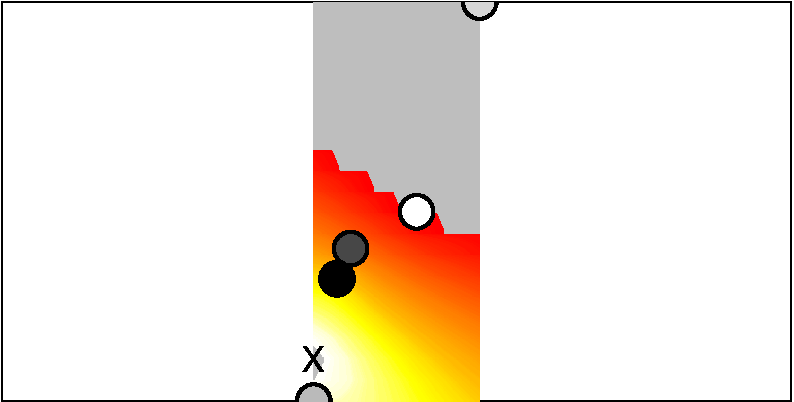
\includegraphics{range_expansion_files/figure-latex/unnamed-chunk-3-1.pdf}

\begin{Shaded}
\begin{Highlighting}[]
\NormalTok{my_psi <-}\StringTok{ }\KeywordTok{as.matrix}\NormalTok{(psi)}
\KeywordTok{rownames}\NormalTok{(my_psi) <-}\StringTok{ }\NormalTok{pop}\OperatorTok{$}\NormalTok{coords}\OperatorTok{$}\NormalTok{pop}
\KeywordTok{colnames}\NormalTok{(my_psi) <-}\StringTok{ }\NormalTok{pop}\OperatorTok{$}\NormalTok{coords}\OperatorTok{$}\NormalTok{pop}
\KeywordTok{max}\NormalTok{(my_psi)}
\end{Highlighting}
\end{Shaded}

\begin{verbatim}
## [1] 0.03659951
\end{verbatim}

\begin{Shaded}
\begin{Highlighting}[]
\CommentTok{# heatmap(my_psi, Rowv = TRUE, symm = TRUE, col = heat.colors(256), margins=c(5,10))}
\CommentTok{# ?heatmap}
\CommentTok{# my_psi$pop1 <- rownames(my_psi)}
\NormalTok{melted_cormat <-}\StringTok{ }\NormalTok{reshape2}\OperatorTok{::}\KeywordTok{melt}\NormalTok{(my_psi, }\DataTypeTok{na.rm =} \OtherTok{TRUE}\NormalTok{)}

\NormalTok{melted_cormat <-}\StringTok{ }\NormalTok{melted_cormat[}\KeywordTok{order}\NormalTok{(melted_cormat}\OperatorTok{$}\NormalTok{value, }\DataTypeTok{decreasing =} \OtherTok{TRUE}\NormalTok{),]}
\NormalTok{melted_cormat}\OperatorTok{$}\NormalTok{Var1 <-}\StringTok{ }\KeywordTok{factor}\NormalTok{(melted_cormat}\OperatorTok{$}\NormalTok{Var1, }\DataTypeTok{levels=}\KeywordTok{unique}\NormalTok{(melted_cormat}\OperatorTok{$}\NormalTok{Var1[}\KeywordTok{order}\NormalTok{(melted_cormat}\OperatorTok{$}\NormalTok{value)]))}
\NormalTok{melted_cormat}\OperatorTok{$}\NormalTok{Var2 <-}\StringTok{ }\KeywordTok{factor}\NormalTok{(melted_cormat}\OperatorTok{$}\NormalTok{Var2, }\DataTypeTok{levels=}\KeywordTok{unique}\NormalTok{(melted_cormat}\OperatorTok{$}\NormalTok{Var2[}\KeywordTok{order}\NormalTok{(melted_cormat}\OperatorTok{$}\NormalTok{value)]))}

\KeywordTok{ggplot}\NormalTok{(}\DataTypeTok{data =} \KeywordTok{filter}\NormalTok{(melted_cormat, value }\OperatorTok{>}\DecValTok{0}\NormalTok{), }\KeywordTok{aes}\NormalTok{(Var1, Var2, }\DataTypeTok{fill =}\NormalTok{ value))}\OperatorTok{+}
\StringTok{  }\KeywordTok{geom_tile}\NormalTok{(}\DataTypeTok{color =} \StringTok{"white"}\NormalTok{)}\OperatorTok{+}
\StringTok{  }\KeywordTok{scale_fill_gradient2}\NormalTok{(}\DataTypeTok{low =} \StringTok{"blue"}\NormalTok{, }\DataTypeTok{high =} \StringTok{"red"}\NormalTok{, }\DataTypeTok{mid =} \StringTok{"white"}\NormalTok{, }
                       \DataTypeTok{midpoint =} \DecValTok{0}\NormalTok{, }\DataTypeTok{limit =} \KeywordTok{c}\NormalTok{(}\DecValTok{0}\NormalTok{,}\KeywordTok{max}\NormalTok{(my_psi)), }\DataTypeTok{space =} \StringTok{"Lab"}\NormalTok{, }
                       \DataTypeTok{name=}\StringTok{"Psi"}\NormalTok{) }\OperatorTok{+}
\StringTok{  }\KeywordTok{xlab}\NormalTok{(}\StringTok{"Psi_1"}\NormalTok{) }\OperatorTok{+}
\StringTok{  }\KeywordTok{ylab}\NormalTok{(}\StringTok{"Psi_2"}\NormalTok{) }\OperatorTok{+}
\StringTok{  }\KeywordTok{theme_minimal}\NormalTok{()}\OperatorTok{+}\StringTok{ }
\StringTok{  }\KeywordTok{theme}\NormalTok{(}\DataTypeTok{axis.text.x =} \KeywordTok{element_text}\NormalTok{(}\DataTypeTok{angle =} \DecValTok{45}\NormalTok{, }\DataTypeTok{vjust =} \DecValTok{1}\NormalTok{, }
                                   \DataTypeTok{size =} \DecValTok{12}\NormalTok{, }\DataTypeTok{hjust =} \DecValTok{1}\NormalTok{))}\OperatorTok{+}
\StringTok{  }\KeywordTok{coord_fixed}\NormalTok{()}
\end{Highlighting}
\end{Shaded}

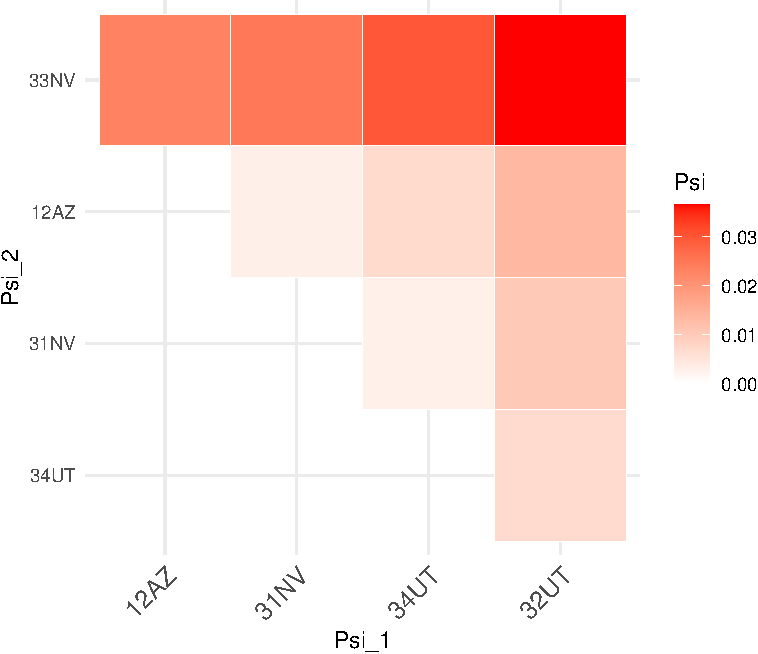
\includegraphics{range_expansion_files/figure-latex/unnamed-chunk-4-1.pdf}

\end{document}
